This chapter looks at the testing performed using trail runner and trail viewer in a non-\gls{crn}. We will go over a set of test cases that were first preformed to validate that trail runner and trail viewer were presenting accurate results. The next set of tests will move toward identifying the minimal length of delay line necessary to evaluate the trail for later implementation as a \gls{crn}. We first cover the methodology we used for the testing and present the results. The chapter concludes with a discussion of the results.

\section{Methodology}
\label{sec:trail_runner_methods}
In this section, we will outline how we verified that trail runner functioned as expected and later used to find the optimal length of delay line. We did the evaluation testing on three trails: test trail 1, test trail 2 (Figure~\ref{fig:test_trails}), and the John Muir Trail (Figure~\ref{fig:johnmuirtrailimage}). We developed a genetic algorithm based off a simple straightforward algorithm proposed by B\"{a}ck~\cite{Baeck2000-co}. A version of this algorithm was already implemented in \gls{deap}, known as \texttt{varAnd}~\cite{Fortin2012-yv}; however, the algorithm did not have all of our desired functionality. Namely, we wanted the ability to monitor the progress of the \gls{ga} in real time, so we used it as a basis for our \gls{ga}. It also did not directly support the selection method we used, $(\mu + \lambda)$ selection~\cite{Schwefel1976-er}. Figure~\ref{fig:ga_flowchart} shows a flowchart of this process discussed that you may find helpful while reading this section.

\begin{figure}[p]
\centering
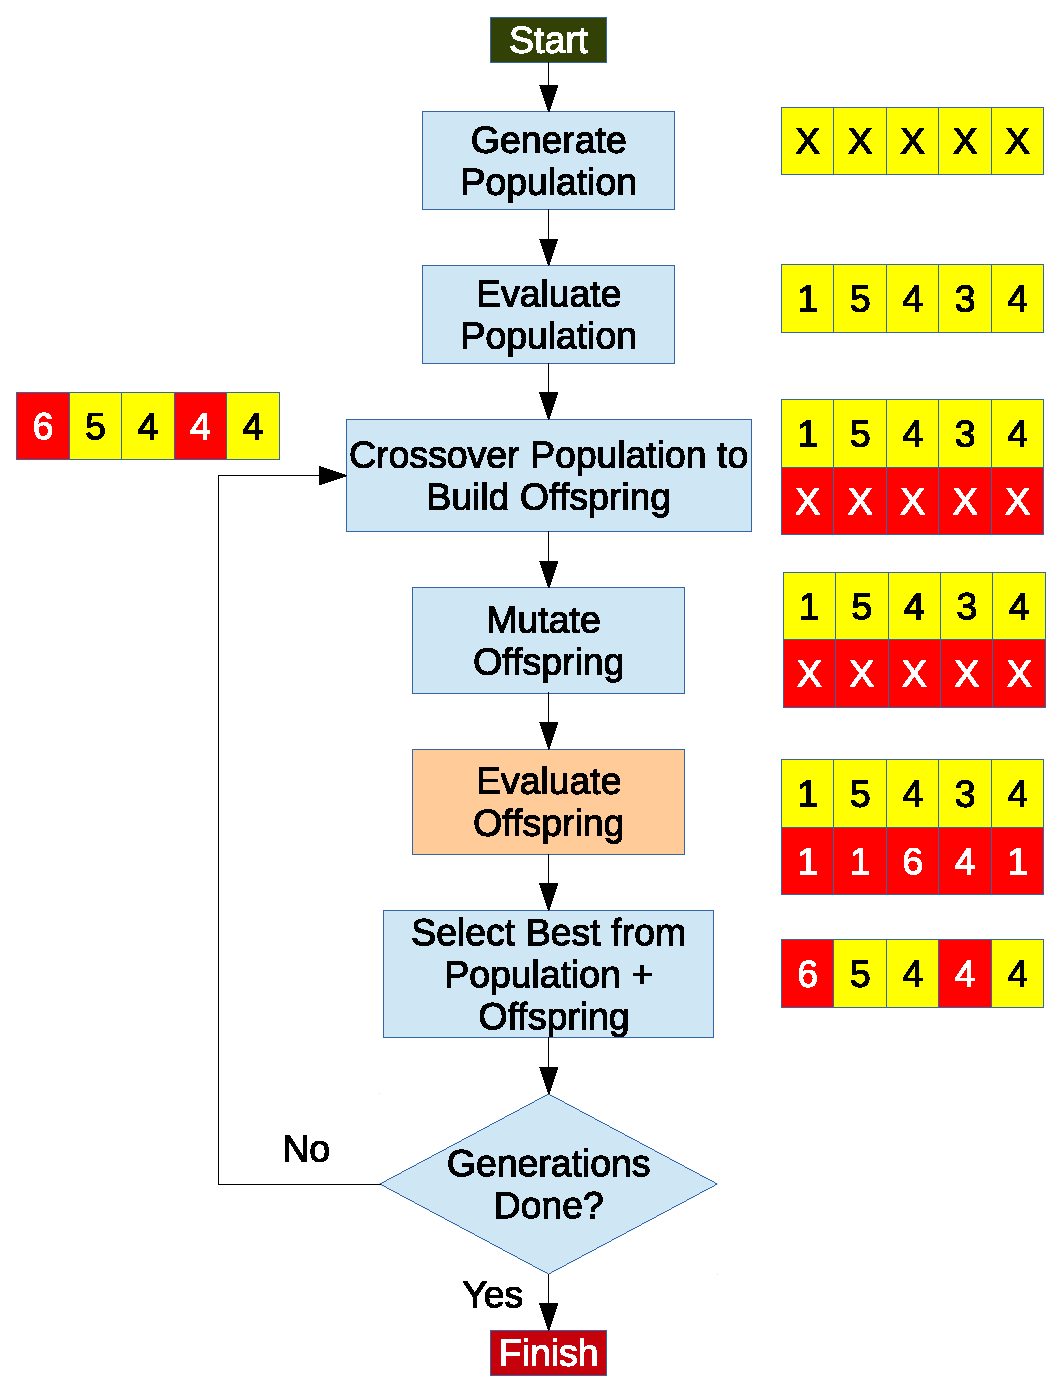
\includegraphics[width=.8\textwidth]{ga_flowchart}
\caption[Genetic Algorithm Flow Chart]{Flowchart of the \gls{ga} used to test the trails. Based off the algorithm proposed by \cite{Baeck2000-co} and \cite{Fortin2012-yv}. The boxes to the right and left each represent an individual through each phase of the \gls{ga}. An $X$ indicates the fitness is unknown and a number represents a fitness (higher is better). The pool to the left of crossover population represents the indivuals selected and looping back on the ``No'' path from ``Generations Done''.}
\label{fig:ga_flowchart}
\end{figure}

The \gls{ga} we used started by generating a population with a size, $P$, defined by the user. The individuals in this pool are a set of real-valued vectors that are in the period between the minimum weight and maximum weight, or $[w_{min}, w_{max}]$. Each of these values corresponded to a weight connecting perceptrons on the \gls{ann}. Each individual is then evaluated to determine their fitness by running them for $M$ moves through the specified trail. The intent was to find all pieces of food before focusing on minimizing the number of foods. We wanted to place greater emphasis on the amount of food consumed, so fitness ($f$) is calculated by:

\begin{equation} \label{eq:fitness_equation}
f = 1.0 \times food\:consumed - 0.1 \times moves\:taken
\end{equation}

Afterwards, we crossover the population with a two-point crossover~\cite{De_Jong1975-wc} with a specified probability of undergoing crossover, $p_x$. If an individual does not get selected for crossover, it is copied to the pool of offspring.

Next, a Gaussian mutation method is used on the pool of offspring because of it's common use for real-valued vectors~\cite{Baeck2000-co}. All individuals enter mutation in this algorithm and each real value of the chromosome is adjusted with a probability of mutation, $p_m$. Then, these offspring are evaluated and assigned their fitnesses before entering selection. Our selection selected the best $P$ individuals from the pool of offspring and the original population. This selection method is also known as $(\mu + \lambda)$~\cite{Schwefel1976-er}. We then continue to repeat this process until one of the three criteria for exiting are met:

\begin{itemize}
\item the user specified number of generations ($G$) are evaluated,
\item all food in the trail is consumed, or
\item or there has been no change in the standard deviation of the mean fitness ($m_g$) of the individual pool for the previous $g$ generations.
\end{itemize}

The final termination criteria was added to save processing time for this task. We found that if the average was stuck at this point for a long period of time. The likelihood of one of these runs with the stuck average proceeding to increase fitness was low. Also, the amount of time in general to solve this problem was rather large so terminating an evaluation that is not progressing is more advantageous than waiting. Note that by terminating when all food is consumed means no optimization for the number of moves taken. The goal was to consume all of the food in the provided number of moves. We will show an example in the results where we terminated a run early with no change in mean fitness.

The algorithm itself had several parameters, such as population, probabilities, and generations, that we must specify. Values were selected based of recent publications as a starting point for evaluation of the \gls{ga}. We selected a population, $P$, of 100 with a probability of crossover, $p_x$, of 0.6 based off work by De Jong et. al.~\cite{De_Jong1991-cq}. For the test trails, we selected a smaller population of 10 to reduce the probability of a solution at generation 1. In other words, we wanted to force the \gls{ga} to operate rather than potentially randomly finding a good candidate on the first run for such a small trail. We selected a probability of mutation, $p_m$, of 0.05 from De Jong's thesis work~\cite{De_Jong1975-wc}. Weights in the range of $[-5.0, 5.0]$ were selected for the neural networks. We set the number of generations ($G$) to a relatively high value of 5000 generations because we generally found that either all food was consumed or the value of $m_g$ settled and exited early prior to reaching 5000 generations. A summary of these parameters is shown in Table~\ref{tab:testing_run_parameters}.

\begin{table}[ht]
\centering
\begin{tabular}{ll}
\textbf{Parameter}                  & \textbf{Value} \\ \hline
Population ($P$)                    & 100 (10 for Test Trail)   \\
Probability of Mutation ($p_m$)     & 0.05  \\
Probability of Crossover ($p_x$)    & 0.6  \\
Generations ($G$)                   & 5000  \\
Mean Fitness Generations ($g$)      & 300  \\
Weight Range ($[w_{min}, w_{max}]$) & $[-5.0, 5.0]$
\end{tabular}
\caption[Summary of GA Parameters for Test Runs]{This table summarizes the parameters used for the test runs in this chapter. The population and probabilities are based of work by De Jong in \cite{De_Jong1991-cq} and \cite{De_Jong1975-wc}. The generations, mean fitness generations, and weight range are set to allow ample exploration.}
\label{tab:testing_run_parameters}
\end{table}

Using this \gls{ga} configuration, we tested the \gls{ga} against test trail 1, test trail 2, John Muir trail, and performance evaluations on the Santa Fe trail. For each trail, we limited the number of moves to 10, 20, 100, and 200, respectively. The test trail values is based off the minimum number of moves necessary plus a small overhead. The values for the John Muir and Santa Fe trail are the same used by Jefferson~\cite{Jefferson1992-ph} and Koza~\cite{Koza1992-xs}. These values are summarized in Table~\ref{tab:testing_moves_limit}. For this verification exercise, we use a neural network that is the same layout as the one Jefferson used to original solve the John Muir trail. 

\begin{table}[ht]
\centering
\begin{tabular}{lcccc}
\textbf{Trail}  & $\bm{M}$  & \textbf{Min. Moves} & \textbf{Food} & \textbf{Max. Fitness} \\ \hline
Test 1    & 10  & 7   & 5  & 4.3 \\ 
Test 2    & 20  & 14  & 9  & 7.6 \\
John Muir & 200 & 147 & 89 & 74.3 \\
Santa Fe  & 400 & 165 & 89 & 72.5
\end{tabular}
\caption[Moves Limits for Test Runs]{We show the statistics for the trails used in this chapter. The move limits ($M$) for test trails are slightly more than the minimum number of moves for each and the John Muir and Santa Fe the same values as Jefferson and Koza. The maximum fitness is calculated with Equation~\ref{eq:fitness_equation}.}
\label{tab:testing_moves_limit}
\end{table}

Next, we were looking to find the minimal length of delay line connected to the smallest \gls{ann} for consuming the most amount of food in the trail. To reduce the time required for each evolution, we started evaluation on three trails that are a subset of the Santa Fe trail~\cite{Koza1992-xs} as well as testing on the full trail. The Santa Fe trail was selected as the main evaluation trail in a chemistry because Koza claimed it is a more difficult trial. It is also a more common trail in literature today for testing. Figure~\ref{fig:sft_segments} show segments 1, 2, and 3 of the Santa Fe trail. They were extracted as the first portions of the full Santa Fe trail that the agent would normally navigate through.

\begin{figure}
\centering
\begin{subfigure}[b]{.5\textwidth}
    \centering
    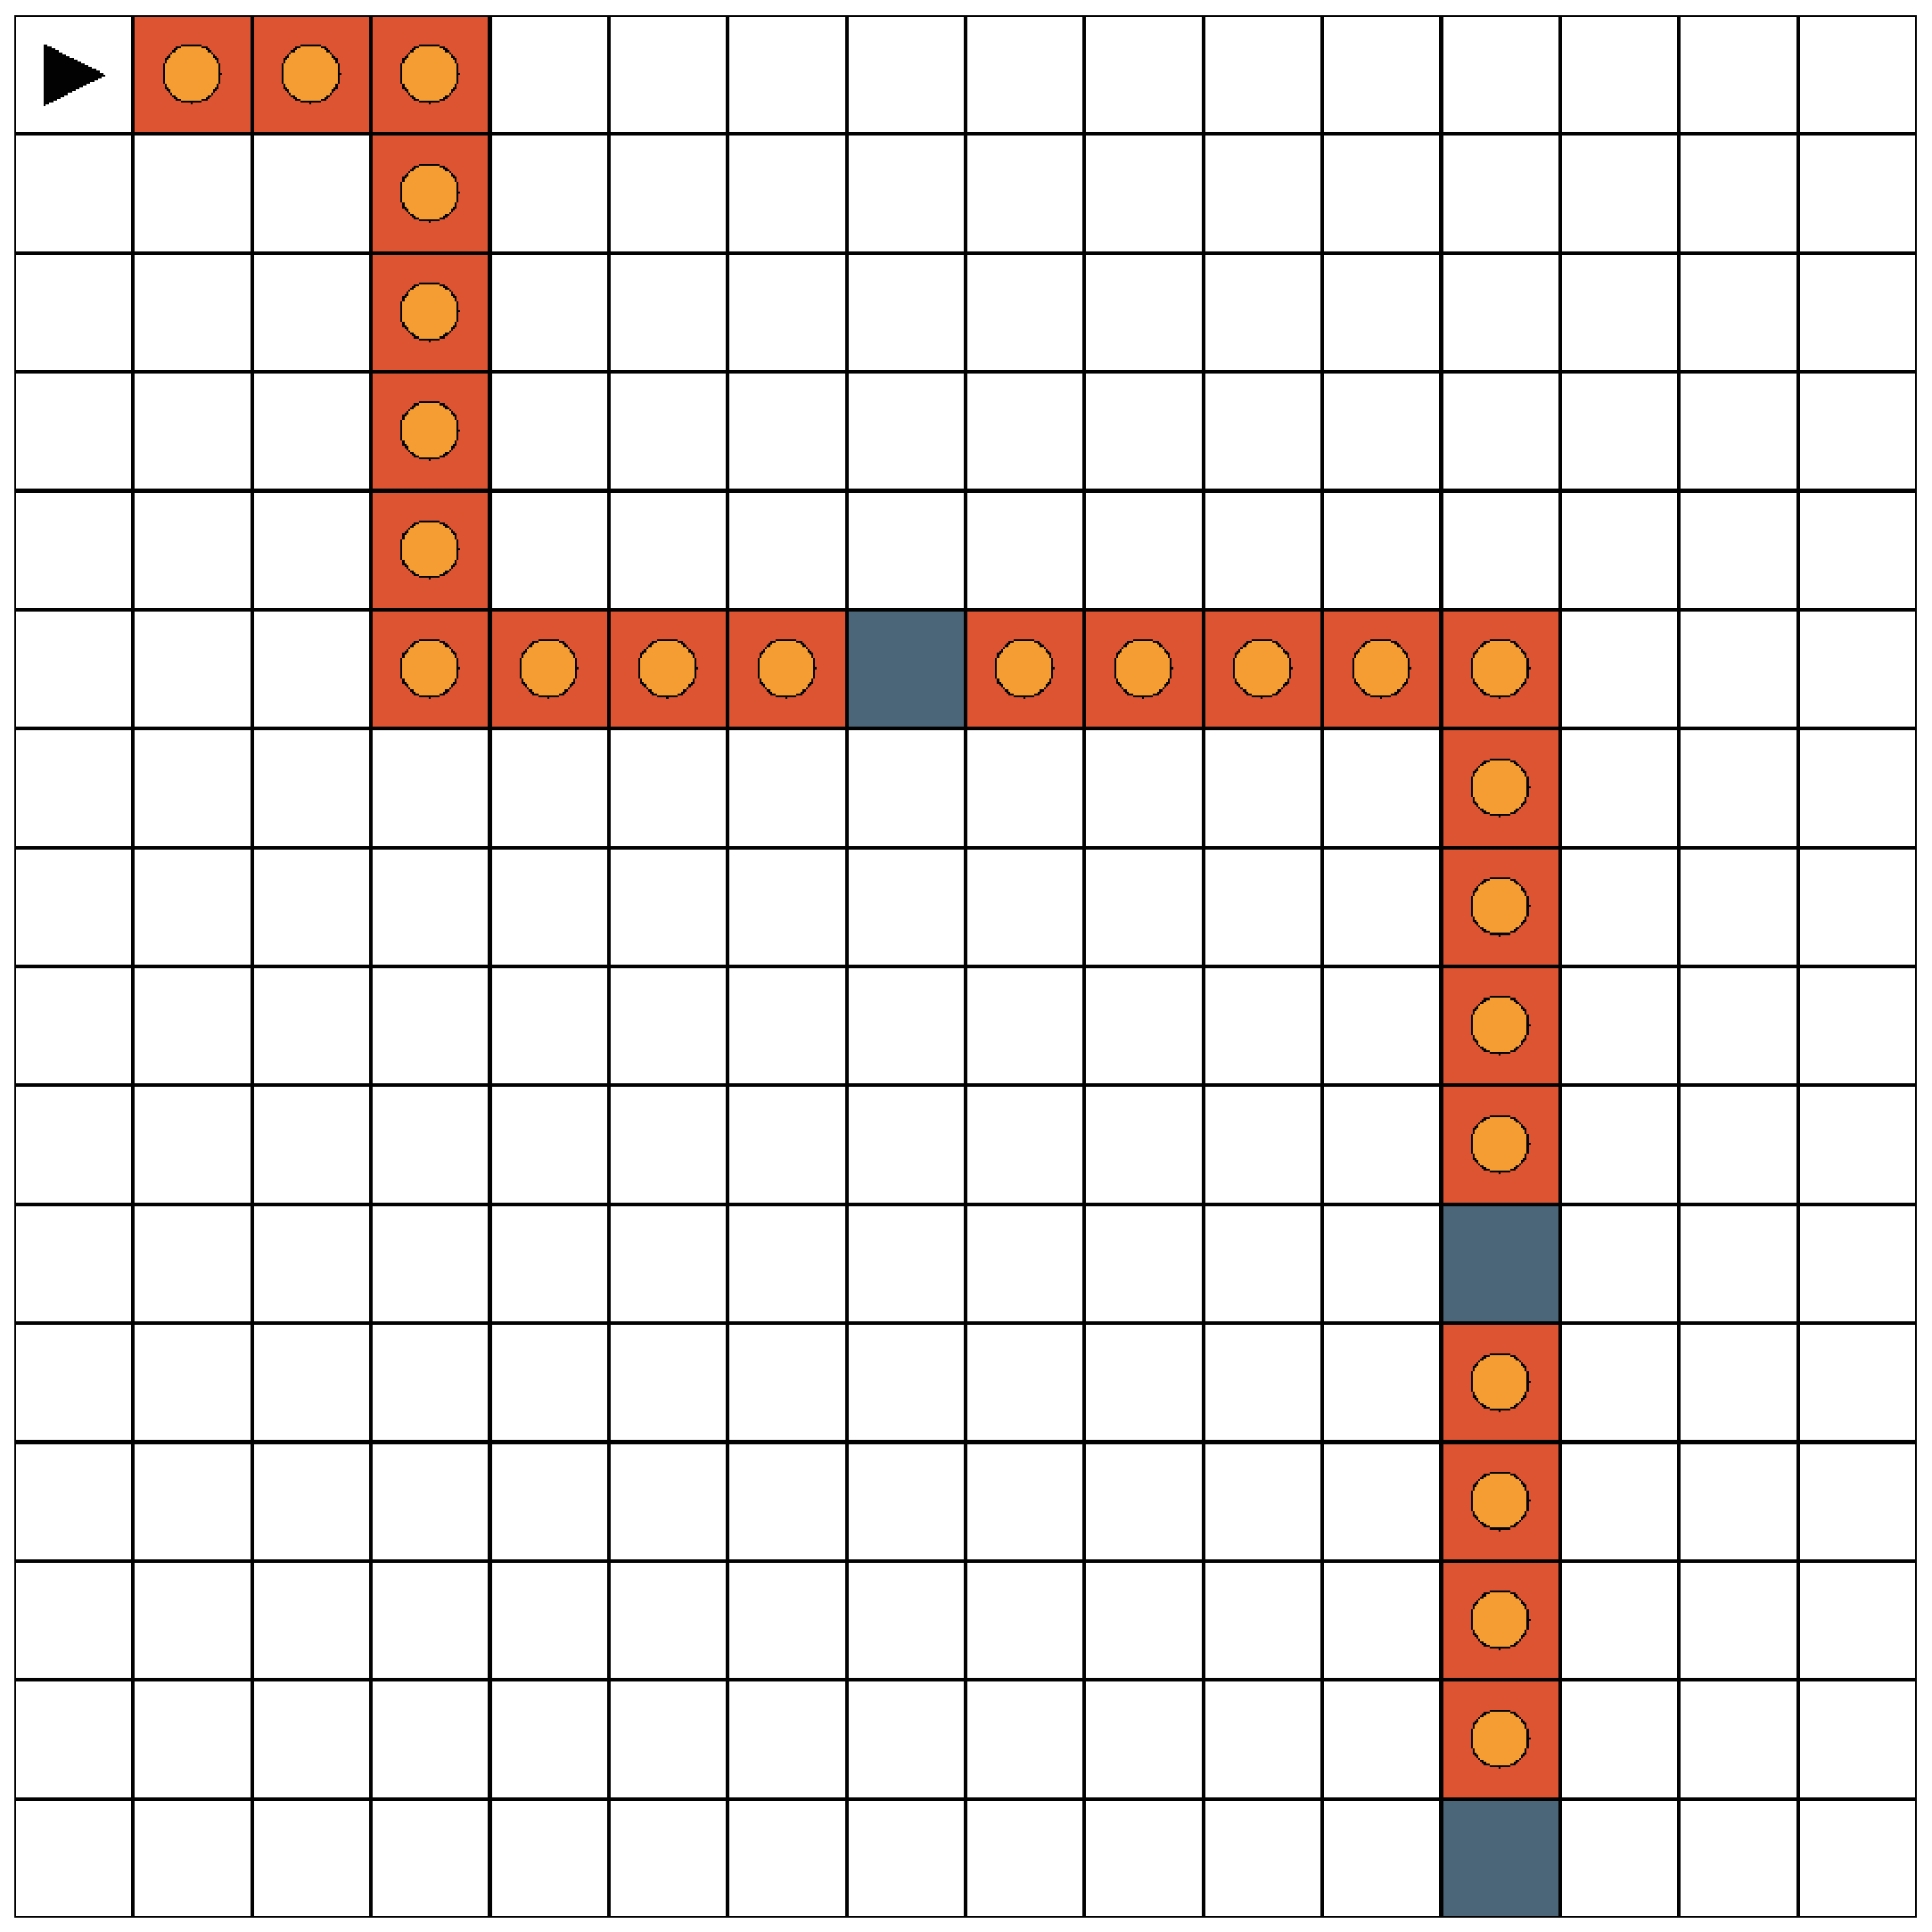
\includegraphics[width=0.5\linewidth]{santa_fe_seg1_17}
    \caption{Santa Fe Trail Segment 1 (Easy)}
    \label{fig:sft_seg1}
\end{subfigure}%
\begin{subfigure}[b]{.5\textwidth}
    \centering
    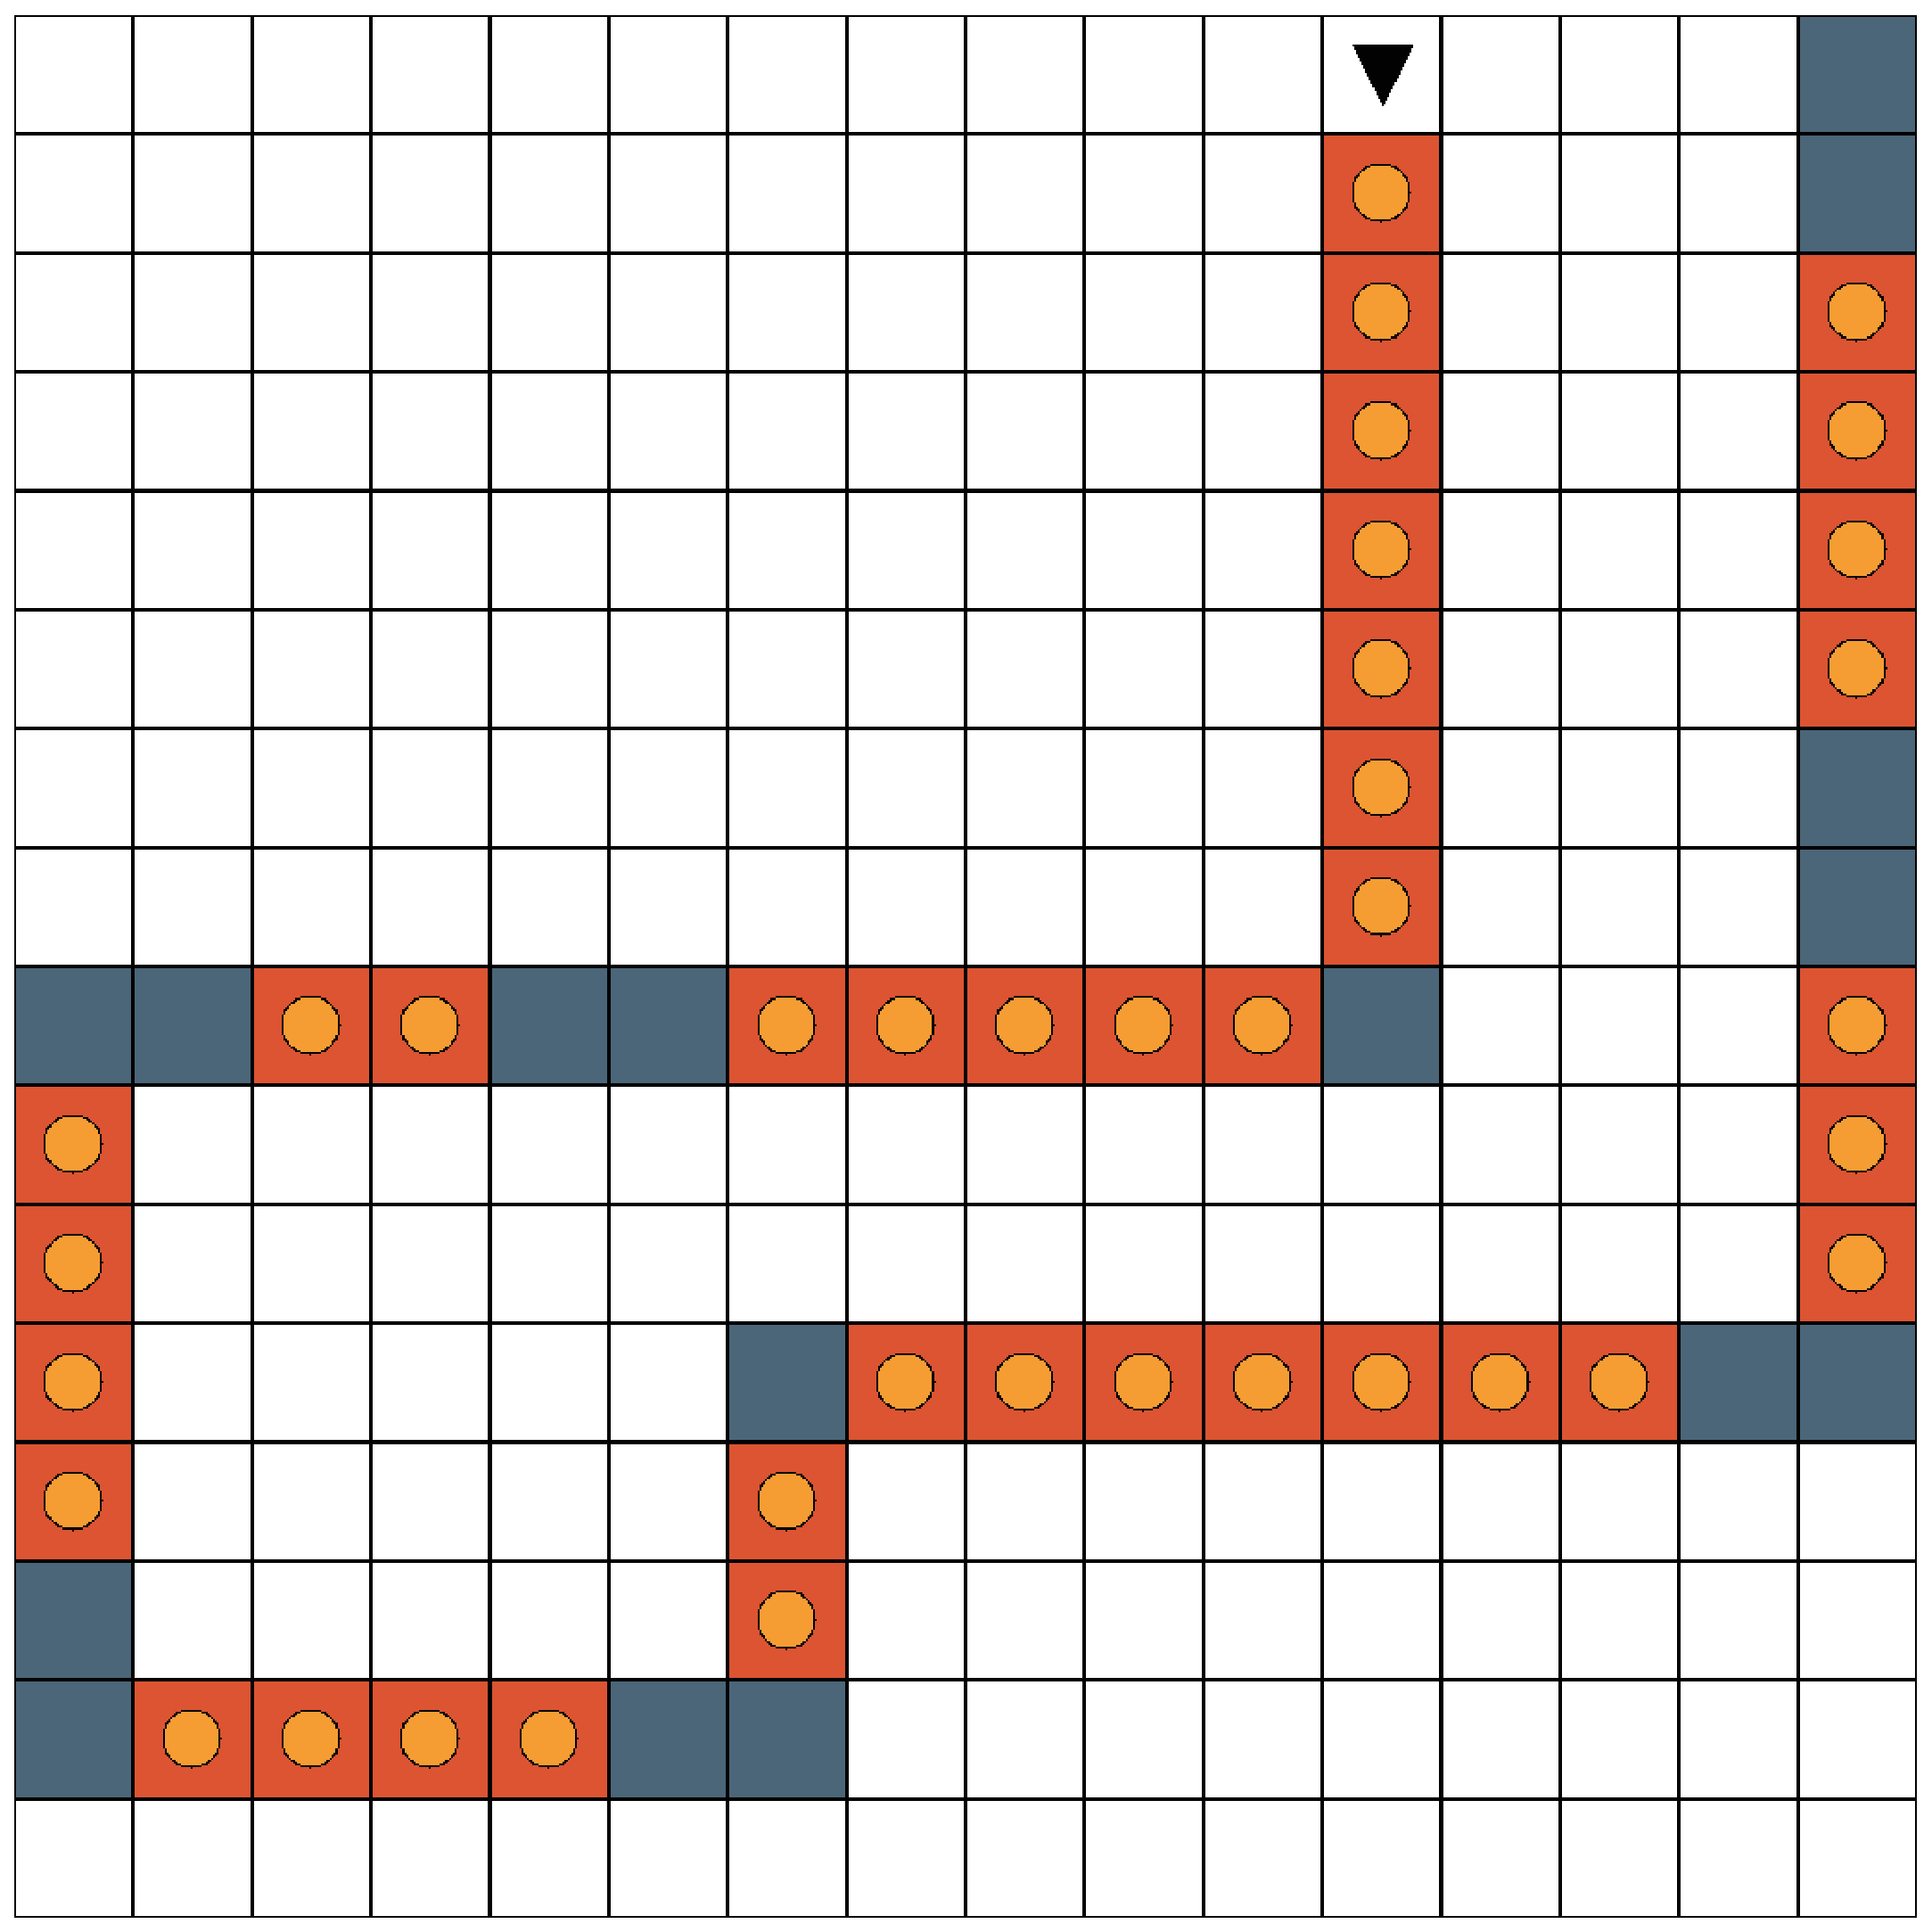
\includegraphics[width=0.5\linewidth]{santa_fe_seg3_19}
    \caption{Santa Fe Trail Segment 3 (Medium)}
    \label{fig:sft_seg3}
\end{subfigure}
\\
\begin{subfigure}[b]{0.5\textwidth}
    \centering
    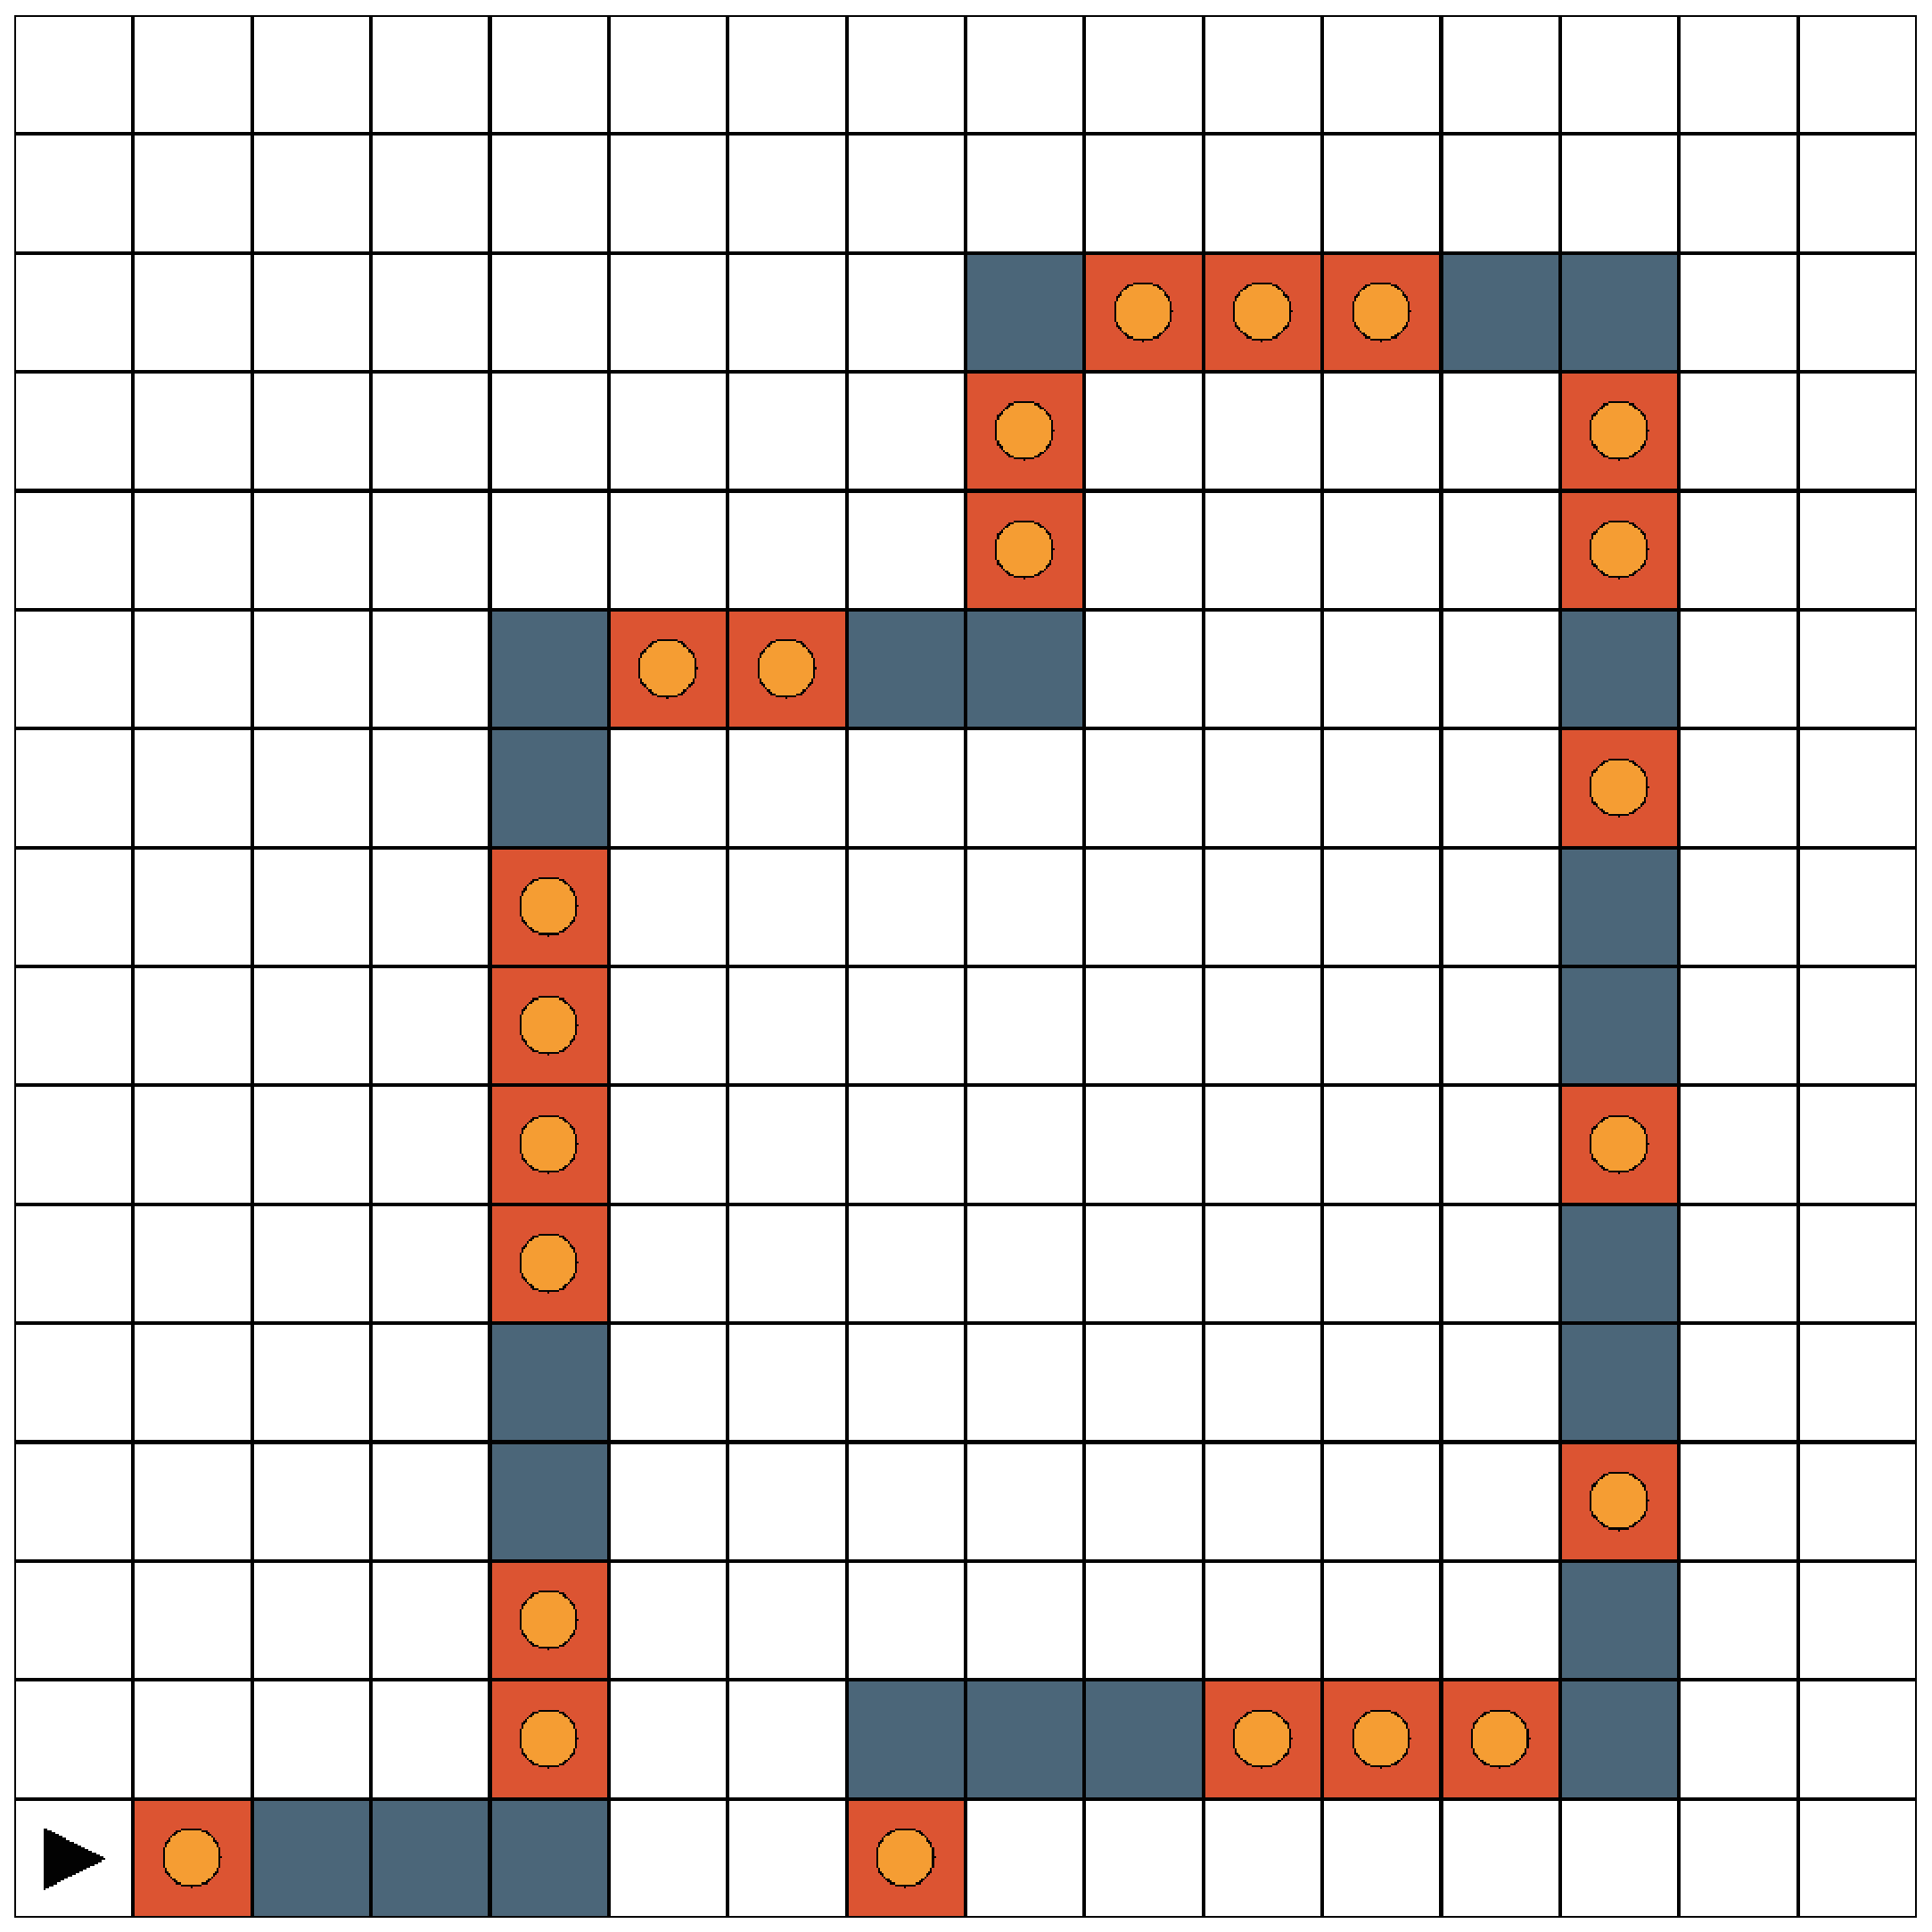
\includegraphics[width=0.5\linewidth]{santa_fe_seg2_18}
    \caption{Santa Fe Trail Segment 2 (Hard)}
    \label{fig:sft_seg2}
\end{subfigure}
\caption[Three Santa Fe Trail Segments]{The three trails with increasing difficult that were used for the delay line length optimization. The number of gaps and turns increases with each trail is the determination for the difficulty.}
\label{fig:sft_segments}
\end{figure}

We used the same \gls{ga} configuration as mentioned above. The moves limit was divided by four ($M = 400 / 4 = 100$) since each trail segment represents a 16 x 16 area which is a quarter of the full Santa Fe trail. Keeping all other parameters the same, we then started going across delay line lengths of $N=2$ all the way up to $N=16$ to search for the minimal length of delay line. 

Like Jefferson's neural network, we had to have a ``food ahead'' and ``not food ahead'' to activate the \gls{ann} in the case of no food ahead. Every delay line segment required two input nodes to hold values. An example \gls{ann} with a delay line of length two is shown in Figure~\ref{fig:trail_ann_w_dl2}. There are a couple of changes from the neural network originally used by Jefferson (see Figure~\ref{fig:jefferson_original_nn}). Our experiments found that only one hidden node in the \gls{ann} was sufficient to solve the task when paired with a delay line. Like Jefferson and Koza, we also found that the ``None'' (meaning no move) output from the \gls{ann} was not used by the best individuals~\cite{Jefferson1992-ph}~\cite{Koza1992-xs}. So, the number of total nodes in the system is represented by Equation~\ref{eq:node_count_eq}.

\begin{equation} \label{eq:node_count_eq}
n = 2 \times delay\:line\:length + 4
\end{equation}

\begin{figure}
\centering
\begin{tikzpicture}[->,draw=black!100, node distance=\layerseptikznn]
    % Based off code form http://www.texample.net/tikz/examples/neural-network/
    \tikzstyle{every pin edge}=[<-,shorten <=1pt]
    \tikzstyle{neuron}=[circle,draw=black!50,fill=white!25,minimum size=25pt,inner sep=0pt]
    \tikzstyle{input neuron}=[neuron, draw=black!50, fill=Accent-5-1];
    \tikzstyle{output neuron}=[neuron, draw=black!50, fill=Accent-5-3];
    \tikzstyle{blank neuron}=[neuron, draw=white!50, fill=white!50];
    \tikzstyle{hidden neuron}=[neuron, draw=black!50, fill=Accent-5-2];
    \tikzstyle{annot} = [text width=4em, text centered]
    \tikzstyle{dlbox}=[rectangle,draw=black!50,fill=Accent-5-4];
    \tikzstyle{input value}=[circle,draw=black!50,fill=Accent-5-5!50,minimum size=25pt,inner sep=0pt];

    % Draw the input layer nodes
    \node[input neuron] (I-1) at (0,-2) {};
    \node[input neuron] (I-2) at (0,-3) {};
    \node[input neuron] (I-3) at (0,-4) {};
    \node[input neuron] (I-4) at (0,-5) {};
    
    % Draw the delay line
    \node[input value] (X-1) at (-\layerseptikznn, -2) {X};
    \node[dlbox] (DL-1) at (-\layerseptikznn, -3) {X[0]};
    \node[dlbox] (DL-2) at (-\layerseptikznn, -4) {X[-1]};
    
    % Connect the delay line to itself and the input layer.
    \draw[->, draw=black!100] (X-1) edge (DL-1);
    \draw[->, draw=black!100] (DL-1) edge (DL-2);
    \draw[->, draw=black!100] (DL-1) edge (I-1);
    \draw[->, draw=red!100] (DL-1) edge (I-2);
    \draw[->, draw=black!100] (DL-2) edge (I-3);
    \draw[->, draw=red!100] (DL-2) edge (I-4);
            
    
    % Draw the hidden layer nodes
        \path[yshift=0.5cm]
            node[hidden neuron] (H-1) at (\layerseptikznn, -4) {H1};

    % Draw the output layer node
        \path node[output neuron, pin={[pin edge={->}]right:Forward}] 
                (O-2) at (\layerseptikznn * 2, -2) {};
        \path node[output neuron, pin={[pin edge={->}]right:Left}] 
                (O-3) at (\layerseptikznn * 2, -3) {};
        \path node[output neuron, pin={[pin edge={->}]right:Right}] 
                (O-4) at (\layerseptikznn * 2, -4) {};
        \path node[blank neuron] 
                (O-5) at (\layerseptikznn * 2, -5) {};

    % Connect every node in the input layer with every node in the
    % hidden layer.
    \foreach \source in {1,...,4}
            \path (I-\source) edge (H-1);
            
    \draw[-, draw=violet!100, thick](I-1) -- ($ (I-1) !.75! (O-2) $);
    \draw[-, draw=violet!100, thick](I-2) -- ($ (I-2) !.75! (O-3) $);
    \draw[-, draw=violet!100, thick](I-3) -- ($ (I-3) !.75! (O-4) $);
    \draw[-, draw=violet!100, thick](I-4) -- ($ (I-4) !.75! (O-5) $);
            
    \foreach \dest in {2,...,4}{
        \draw[->, draw=violet!100] ($ (I-1) !.75! (O-2) $) -- (O-\dest.west);
        \draw[->, draw=violet!100] ($ (I-2) !.75! (O-3) $) -- (O-\dest.west);
        \draw[->, draw=violet!100] ($ (I-3) !.75! (O-4) $) -- (O-\dest.west);
        \draw[->, draw=violet!100] ($ (I-4) !.75! (O-5) $) -- (O-\dest.west);
    }

    % Connect every node in the hidden layer with the output layer
    \foreach \dest in {2,...,4}
        \path (H-1) edge (O-\dest);

    % Annotate the layers
    \node[annot,above of=H-1, node distance=3cm] (hl) {Hidden layer};
    \node[annot,left of=hl] {Input layer};
    \node[annot,right of=hl] {Output layer};
\end{tikzpicture}
\caption[Delay Line with ANN for Trails]{This figure shows the \gls{ann} combined with a 2-input ($N=2$) delay line (on left). This feedforward \gls{ann} has full connections from the input to the hidden layer, input to the output layer, and hidden to the output layer. They delay line has two input neurons for each stage: one that is the actual value (black line) and one that is the inverted value (red line) of if there is food ahead. Values shift down the delay line where $X[0]$ represents the current input and $X[-1]$ represents the previous input.}
\label{fig:trail_ann_w_dl2}
\end{figure}

\section{Results}
\label{sec:tools_testing_results}
This presents the results from running testing against test trail 1, test trail 2, John Muir trail, Santa Fe trail, and the three segments. For all of the food consumption plots in this section, ``Max'' shows the food consumed by the best individual, ``Min'' shows the food consumed by the worst individual, and the average of the maximum of the entire population represented by ``Avg''. ``Available'' shows the maximum amount of food available in the trail. 

The first set of results are from test trail 1. Test trail 1 was configured to run with the configuration specified in tables~\ref{tab:testing_run_parameters} and \ref{tab:testing_moves_limit}. We executed a small set of runs (five) with the same configuration. In many cases, an optimal \gls{ga} was found after the first couple generations, but we have presented one here that has a diverse population with varying maximum, mean, and minimum. Figure~\ref{fig:trail1_food_consumed} shows the food consumed versus generations and Figure~\ref{fig:trail1_final_gen} shows the path that the agent at elite individual at the final generation (eight in this case) took to consume the maximum amount of food.

\begin{figure}[ht]
\centering
\begin{tikzpicture}
    \begin{axis}[
    xlabel={Generation},
    ylabel={Food Consumed},
    xticklabel style={/pgf/number format/fixed},
    cycle multi list={Mark-Dark2-4},
    legend style={
        cells={anchor=east},
        legend pos=south east,
    },
    scale only axis, % The height and width argument only apply to the actual axis
    height=7.313cm,
    width=13cm,
    every axis post/.style={
        thick,
    },
    ]
        \addplot table [x=Generations, y=Max, col sep=comma] {data/food_run_39212.csv};
        \addplot table [x=Generations, y=Min, col sep=comma] {data/food_run_39212.csv};
        \addplot table [x=Generations, y=Avg, col sep=comma] {data/food_run_39212.csv};
        \addplot[dashed] table [x=Generations, y=Available, col sep=comma] {data/food_run_39212.csv};
        
        \legend{Max, Min, Avg, Available}
    
    \end{axis}
\end{tikzpicture}
\caption[Food Consumed in Test Trail 1]{Plot showing the food consumed over each generation for test trail 1. With this relatively simple trail, it takes only eight generations to find an individual capable of consuming all the food.}
\label{fig:trail1_food_consumed}
\end{figure}

\begin{figure}[ht]
\centering
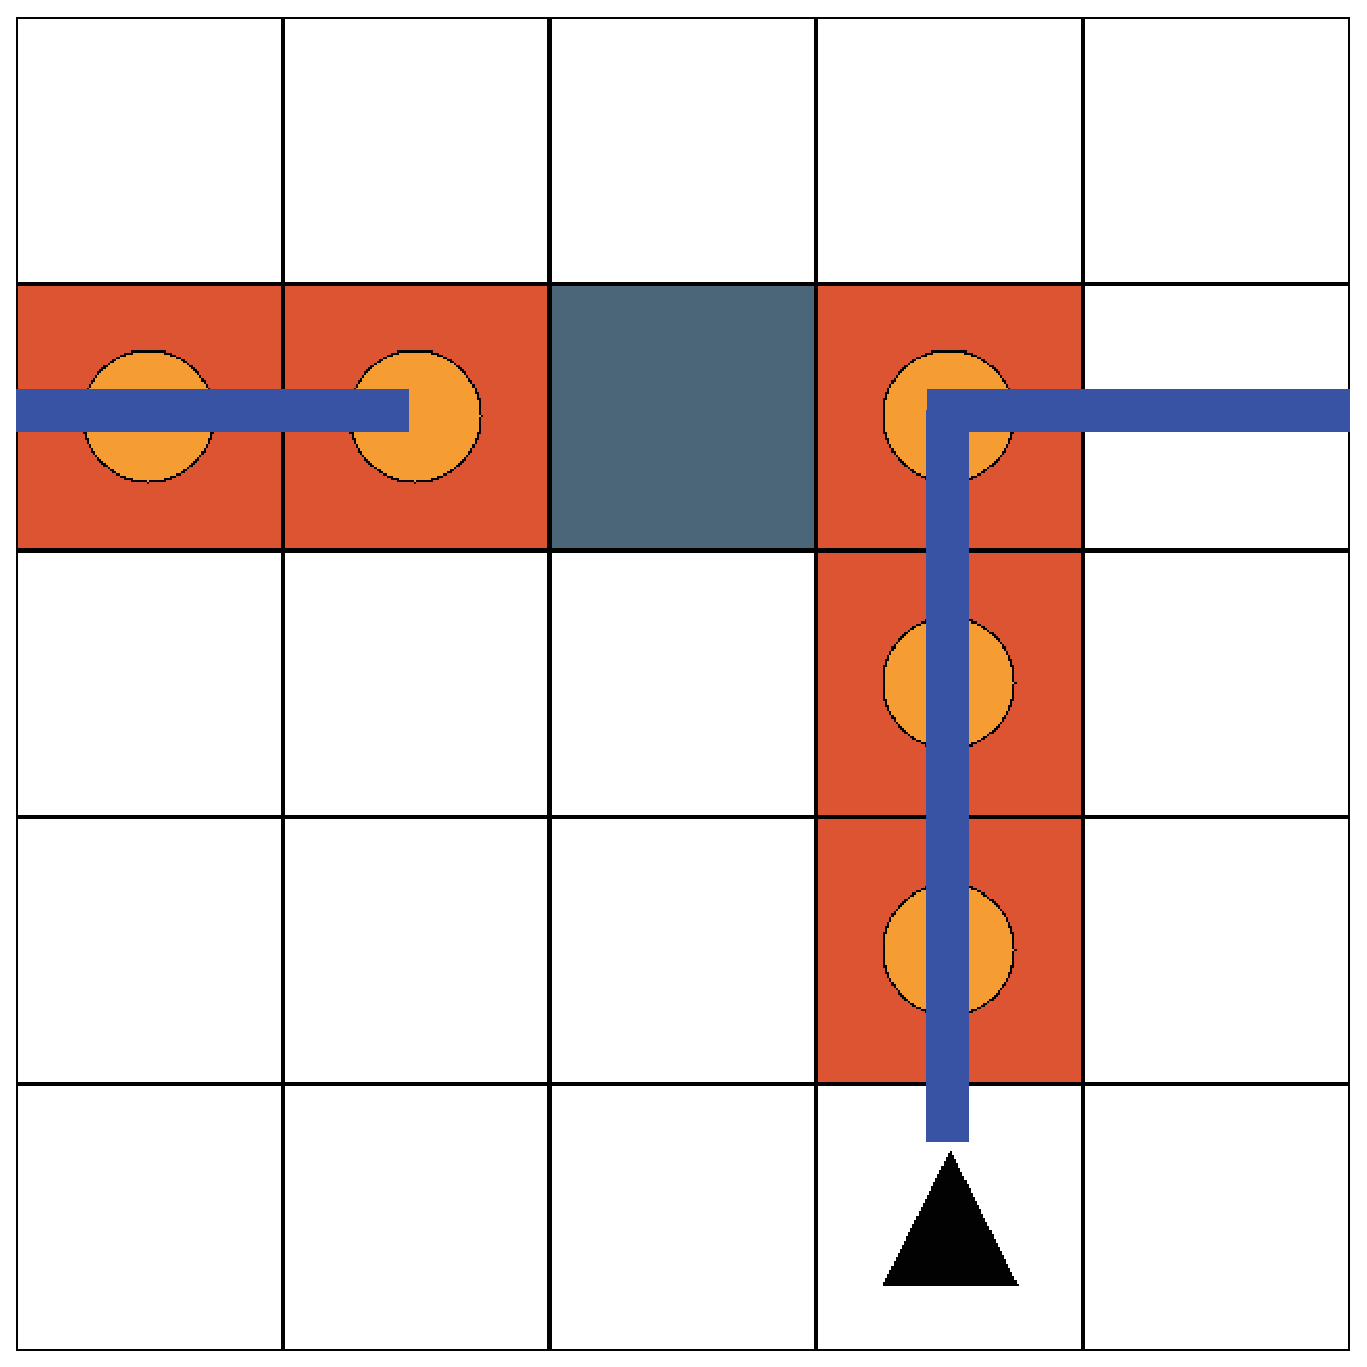
\includegraphics[width=0.25\textwidth]{run39212_t1_gFinal}
\caption[Individual Path in Test Trail 1]{This figure shows the path the best individual took with test trail 1 indicated with the dark line. Note this trail has two optimal paths (left or right at first turn). The particular solution from the \gls{ga} here took the right turn. Video available at \url{http://goo.gl/MUktKs}.}
\label{fig:trail1_final_gen}
\end{figure}

\clearpage
Next, we evaluated test trail 2. Test trail 2 is a slightly more complicated version of test trail 1 featuring two turns, three gaps, and nine pieces of food. This trail is also larger than test trail 1 and the optimal path is to turn left at the first turn versus test trail 1 the agent can turn left or right. This trail was executed with the same configuration with test trail 1 except for allowing twice as many moves, twenty instead of ten. Figure~\ref{fig:trail2_food_consumed} shows how much food the agent consumed and Figure~\ref{fig:trail2_final_gen} shows the path that the final individual took through the maze. Note in this case, the agent actually took extra, unnecessary steps to consume all of the food.

\begin{figure}[ht]
\centering
\begin{tikzpicture}
    \begin{axis}[
    xlabel={Generation},
    ylabel={Food Consumed},
    xticklabel style={/pgf/number format/fixed},
    cycle multi list={Mark-Dark2-4},
    legend style={
        cells={anchor=east},
        legend pos=south east,
    },
    scale only axis, % The height and width argument only apply to the actual axis
    height=7.313cm,
    width=13cm,
    every axis post/.style={
        thick,
    },
    ]
        \addplot table [x=Generations, y=Max, col sep=comma] {data/food_run_39268.csv};
        \addplot table [x=Generations, y=Min, col sep=comma] {data/food_run_39268.csv};
        \addplot table [x=Generations, y=Avg, col sep=comma] {data/food_run_39268.csv};
        \addplot[dashed] table [x=Generations, y=Available, col sep=comma] {data/food_run_39268.csv};
        
        \legend{Max, Min, Avg, Available}
    
    \end{axis}
\end{tikzpicture}
\caption[Food Consumed in Test Trail 2]{Plot of food consumed over each generation on test trail 2. This slightly more complicated trail takes a few more generations, but finds a solution after ten generations.}
\label{fig:trail2_food_consumed}
\end{figure}

\begin{figure}[ht]
\centering
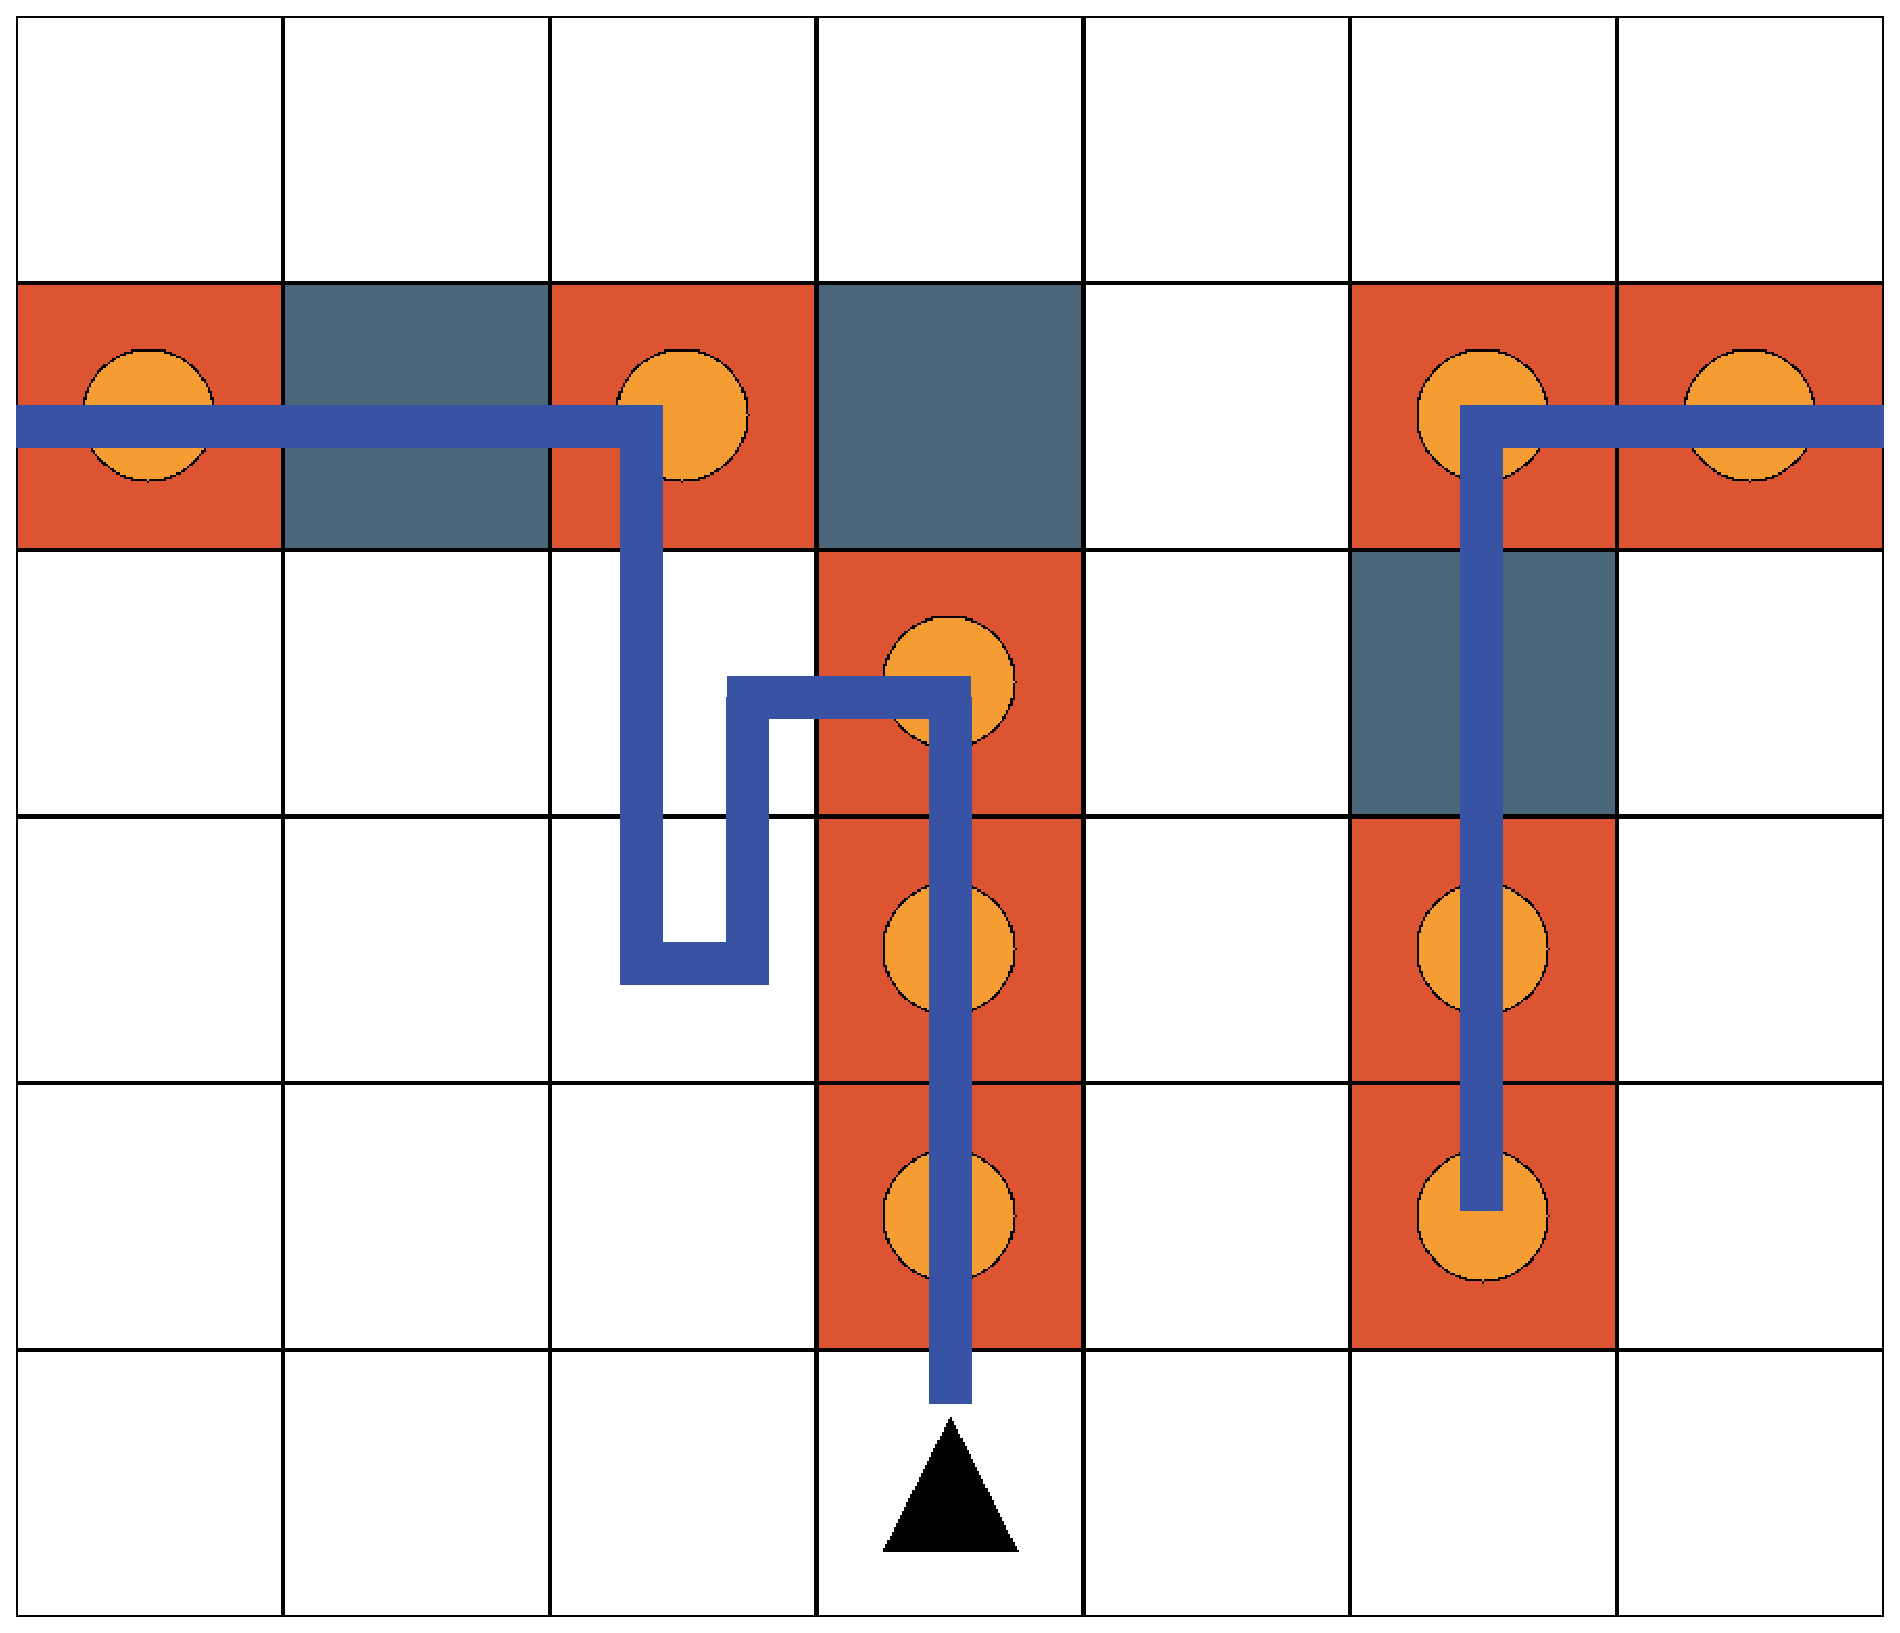
\includegraphics[width=0.25\textwidth]{run39268_t2_gFinal}
\caption[Individual Path in Test Trail 2]{Path of agent consuming food in test trail 2 in final generation. In this case, the ant found a solution consuming all food, but did it with a non-optimal number of moves. As we mentioned before, we stop when a solution that finds all food is found and do not continue to optimize for moves. Video available at \url{http://goo.gl/jDO7p1}.}
\label{fig:trail2_final_gen}
\end{figure}

\clearpage
The next \gls{ga} evaluation was performed on Jefferson's John Muir trail. This is a complicated trail compared to the two test trails and serves as a good starting benchmark for the performance of the \gls{ga}. Figure~\ref{fig:jmt_tr_food_consumed} shows the food consumption over generations. Generation 443 contained an individual that consumed all of the food on the trail. Figure~\ref{fig:jmt_tr_final_gen} shows the path this individual took through the John Muir trail.

\begin{figure}[ht]
\centering
\begin{tikzpicture}
    \begin{axis}[
    xlabel={Generation},
    ylabel={Food Consumed},
    xticklabel style={/pgf/number format/fixed},
    cycle multi list={Mark-Dark2-4},
    legend style={
        cells={anchor=east},
        legend pos=south east,
    },
    scale only axis, % The height and width argument only apply to the actual axis
    height=7.313cm,
    width=13cm,
    mark repeat=20,
    every axis post/.style={
        thick,
    },
    ]
        \addplot table [x=Generations, y=Max, col sep=comma] {data/food_run_39653.csv};
        \addplot table [x=Generations, y=Min, col sep=comma] {data/food_run_39653.csv};
        \addplot table [x=Generations, y=Avg, col sep=comma] {data/food_run_39653.csv};
        \addplot[dashed] table [x=Generations, y=Available, col sep=comma] {data/food_run_39653.csv};
        
        \legend{Max, Min, Avg, Available}
    
    \end{axis}
\end{tikzpicture}
\caption[Food Consumed in John Muir Trail]{Plot showing the consumption of food for each generation on the John Muir trail. This trail took more generations compared to test trail 1 and test trail 2 to reach a solution because of the larger size. It finds a solution after 443 generations.}
\label{fig:jmt_tr_food_consumed}
\end{figure}

\begin{figure}[ht]
\centering
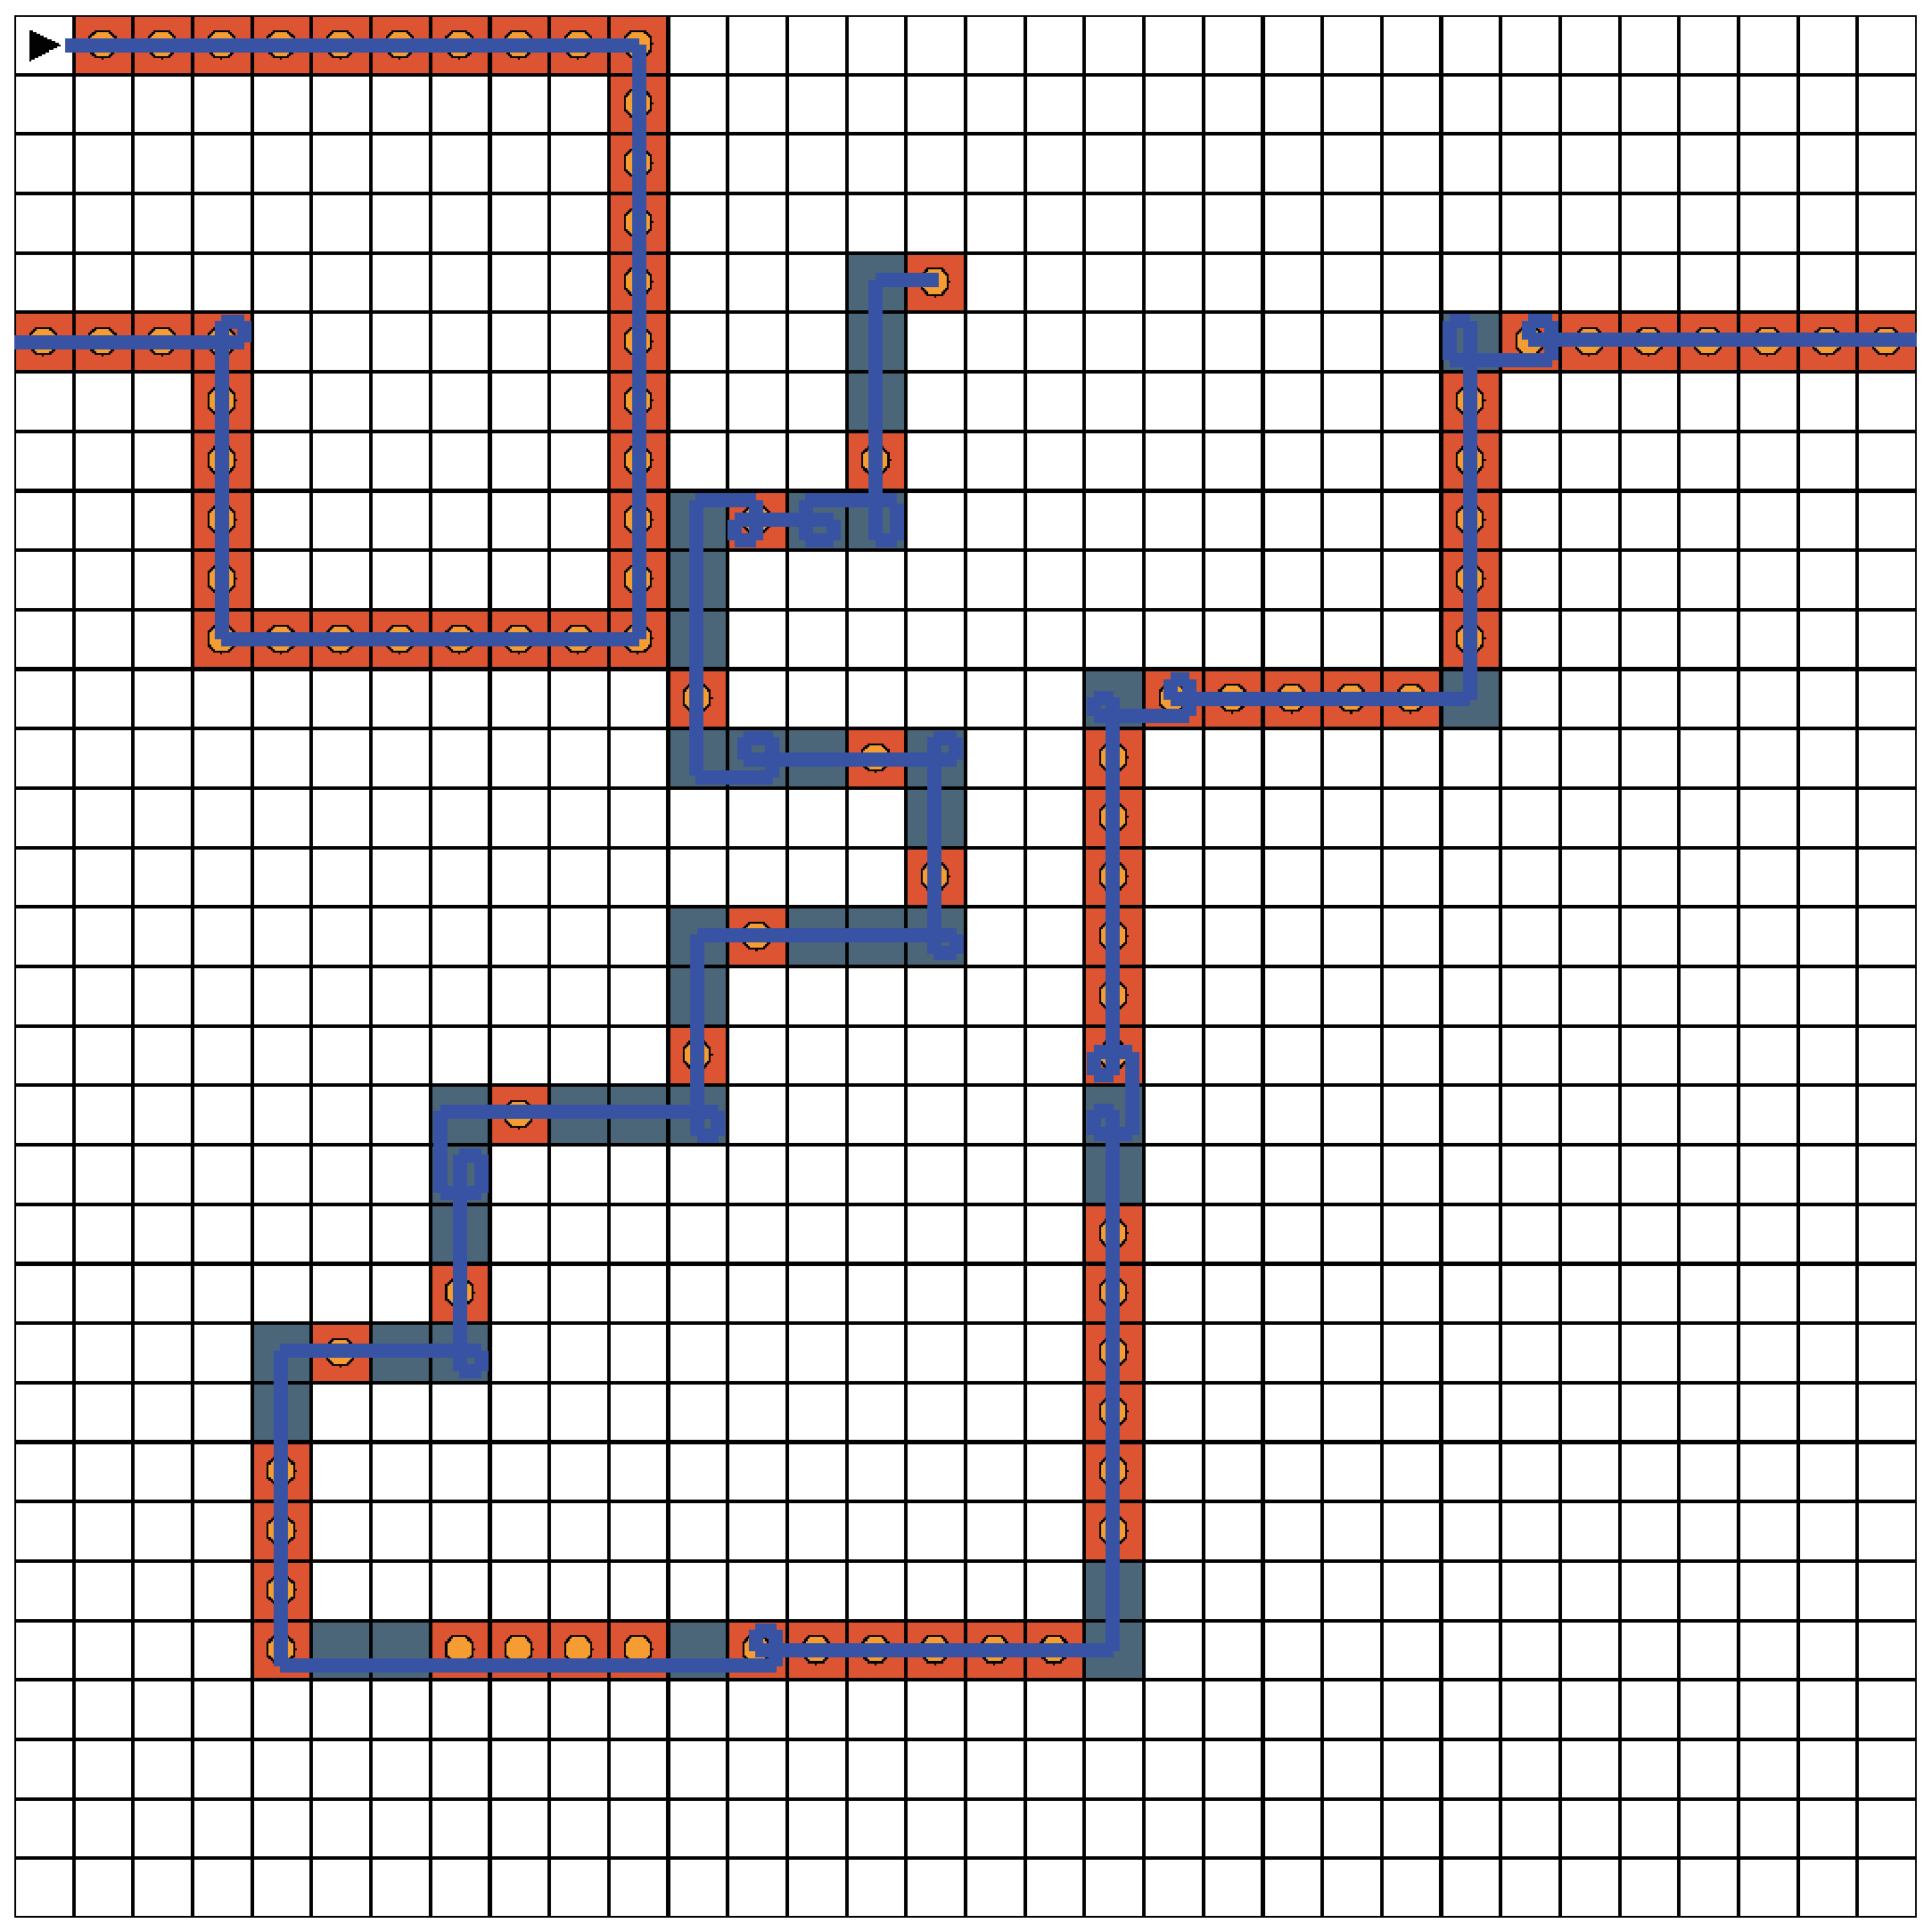
\includegraphics[width=0.95\textwidth]{run39653_t3_gFinal}
\caption[Individual Path in John Muir Trail]{Path of the agent through Santa Fe Trail in final (443) generation. The agent did turn within some squares before moving forward like the first left turn on the trail. This individual required 199 moves and consumed all 89 pieces of food. This individual never took a left turn and only made right turns through the trail. Video available at \url{http://goo.gl/OaGsyh}.}
\label{fig:jmt_tr_final_gen}
\end{figure}

\clearpage
Using the same configuration on the John Muir trail, Figure~\ref{fig:jmt_tr_food_stuck_run} shows an example of a run that was terminated early. This run did not go to completion because there was no change in the standard deviation of the maximum amount of food consumed across the population.

\begin{figure}[ht]
\centering
\begin{tikzpicture}
    \begin{axis}[
    xlabel={Generation},
    ylabel={Food Consumed},
    xticklabel style={/pgf/number format/fixed},
    cycle multi list={Mark-Dark2-4},
    legend style={
        cells={anchor=east},
        legend pos=south east,
    },
    scale only axis, % The height and width argument only apply to the actual axis
    height=7.313cm,
    width=13cm,
    mark repeat=20,
    every axis post/.style={
        thick,
    },
    ]
        \addplot table [x=Generations, y=Max, col sep=comma] {data/food_run_39635.csv};
        \addplot table [x=Generations, y=Min, col sep=comma] {data/food_run_39635.csv};
        \addplot table [x=Generations, y=Avg, col sep=comma] {data/food_run_39635.csv};
        \addplot[dashed] table [x=Generations, y=Available, col sep=comma] {data/food_run_39635.csv};
        
        \legend{Max, Min, Avg, Available}
    
    \end{axis}
\end{tikzpicture}
\caption[Food Consumed in John Muir Trail on Stuck Run]{Plot showing a \gls{ga} run on the John Muir trail that is no longer progressing. This run was terminated early because it did not have a change in the standard deviation of the maximum food conumsed for the previous 300 generations starting at around generation 90. }
\label{fig:jmt_tr_food_stuck_run}
\end{figure}

\clearpage
Now, we will show the results of a performance sweep to see the advantage of using a parallel processing environment, like \gls{scoop}. We performed this evaluation using the Santa Fe Trail and and used the \gls{ga} parameters specified in Table~\ref{tab:testing_run_parameters}. For these trials, we disabled the automatic termination if all food was consumed for a fair comparison. All of these runs ran for the full 100 generations. Then, the number of moves was ran with a value of 100, 200, 300, and 400 across a maximum number of processes of 1, 2, 4, and 8. Figure~\ref{fig:trail_runner_do_benchmark} shows this plot. This benchmark was performed on a DigitalOcean \gls{vps} featuring a 160 GB \gls{ssd}, 16 GB of memory, and an eight core processor~\cite{DigitalOcean_Inc_undated-bc}.

\begin{figure}[ht]
\centering
\begin{tikzpicture}
    \begin{axis}[
    ybar,
    bar width = 0.5cm,
    xlabel={Number of Processes},
    ylabel={Run Time (seconds)},
    legend style={
        cells={anchor=east},
        legend pos=north east,
    },
    scale only axis, % The height and width argument only apply to the actual axis
    symbolic x coords={1, 2, 4, 8},
    enlarge x limits=0.25,
    enlarge y limits=false,
    ymin=0,
    ymax=700,
    xtick=data,
    height=7.313cm,
    width=13cm,
    area legend
    ]
        \addlegendimage{empty legend};
        \addplot [fill={Accent-4-1}] coordinates {(1, 168) (2, 107) (4, 77) (8, 50)};
        
        \addplot [fill={Accent-4-2}, 
            postaction={
                pattern=horizontal lines,
                pattern color=black!50,
            }] coordinates {(1, 317) (2, 193) (4, 116) (8, 81)};
            
        \addplot [fill={Accent-4-3}, postaction={
                pattern=north east lines,
                pattern color=black!50,
            }] coordinates {(1, 468) (2, 266) (4, 167) (8, 108)};
        \addplot [fill={Accent-4-4}, postaction={
                pattern=grid,
                pattern color=black!50,
            }] coordinates {(1, 623) (2, 338) (4, 210) (8, 131)};
        
        \legend{\textbf{Max. Moves}, 100, 200, 300, 400}
    
    \end{axis}
\end{tikzpicture}
\caption[Run Time Benchmark of Trail Runner]{Run time benchmark for trail runner on Santa Fe trail. Benchmark swept the number of processes and maximum number of moves to collect time for each one. Notice how more processes speeds up the simulation and more moves requires more time to process.}
\label{fig:trail_runner_do_benchmark}
\end{figure}

\clearpage
Figure~\ref{fig:sft_none_evidence_plot} shows a run where the ``None'' move option was enabled to show how it is not used by the best individual at the end of the run. This run goes for 89 generations until an individual evolves that consumes all pieces of food. This was performed on the full Santa Fe trail.

\begin{figure}[hbt]
\centering
\begin{tikzpicture}
    \begin{axis}[
    xlabel={Generation},
    ylabel={Number of Moves},
    xticklabel style={/pgf/number format/fixed},
    cycle multi list={Mark-Dark2-4},
    legend style={
        cells={anchor=east},
        legend pos=north east,
        legend columns=2,
    },
    scale only axis, % The height and width argument only apply to the actual axis
    height=7.313cm,
    width=13cm,
    mark repeat=10,
    every axis post/.style={
        thick,
    },
    ]
        \addplot table [x=Generations, y=Left, col sep=comma] {data/moves_dir_run_39527.csv};
        \addplot table [x=Generations, y=Right, col sep=comma] {data/moves_dir_run_39527.csv};
        \addplot table [x=Generations, y=Forward, col sep=comma] {data/moves_dir_run_39527.csv};
        \addplot table [x=Generations, y=None, col sep=comma] {data/moves_dir_run_39527.csv};
        
        \legend{Left, Right, Forward, None}
    
    \end{axis}
\end{tikzpicture}
\caption[Moves Type in Santa Fe Trail]{Plot showing the moves the best individual took over a run of 89 moves where it ended with an individual who consumed all food. Notice how the individuals starting around generation 70 took no ``None'' actions. This individual also evolved a final strategy where it only took left turns. This was a common theme in the Jefferson \gls{ann} solutions.}
\label{fig:sft_none_evidence_plot}
\end{figure}

\clearpage
We next swept the delay line length from $N=2$ up to $N=16$ on each of the three segments of the Santa Fe Trail. Figure~\ref{fig:sft_segment_dl_len_sweeps} shows the results on the food collected by the best individual for each of the three segments and the full Santa Fe trail. This chart is showing the best individual run out of a minimum of 70 \gls{ga} evaluations for every delay line length and every trail segment. There are a minimum of 25 evaluations for each length of the full Santa Fe trail. The values are normalized by dividing the food obtained by the maximum amount of food on the trail.

\begin{figure}[hbt]
\centering
\begin{tikzpicture}
    \begin{axis}[
    xlabel={Delay Line Length},
    ylabel={Norm. Food Consumed},
    xticklabel style={/pgf/number format/fixed},
    cycle multi list={Mark-Dark2-4},
    legend style={
        cells={anchor=east},
        legend pos=south east,
    },
    scale only axis, % The height and width argument only apply to the actual axis
    height=7.313cm,
    width=13cm,
    every axis post/.style={
        thick,
    },
    ]
        \addplot table [x=Delay Line Length, y=max_norm, col sep=comma] {data/sweep_trail17.csv};
        \addplot table [x=Delay Line Length, y=max_norm, col sep=comma] {data/sweep_trail19.csv};
        \addplot table [x=Delay Line Length, y=max_norm, col sep=comma] {data/sweep_trail18.csv};
        \addplot table [x=Delay Line Length, y=max_norm, col sep=comma] {data/sweep_trail5.csv};
        
        \legend{Easy (Segment 1), Medium (Segment 2), Hard (Segment 3), Full Trail}
    
    \end{axis}
\end{tikzpicture}
\caption[Maximum Food Gathered by Varying Delay Line Length]{This plot shows the normalized food gathered by the best individual for a given run with varying delay line lengths. Each segment is a subset of the Santa Fe trail. Values were normalized by dividing the food gathered by maximum available for each trail. Notice how a \gls{mdl} of length 2 or 3 is not sufficient. At length 4, the agent start collecting at least 60\% of the available food for all segments and the full trail. The full trail is a more difficult task compared to the segments because there is a much larger trail to explore provided a larger chance for the agent to make poor moves.}
\label{fig:sft_segment_dl_len_sweeps}
\end{figure}

\clearpage
Figure~\ref{fig:sft_easy_segment_mean_dl_len_sweeps}, Figure~\ref{fig:sft_med_segment_mean_dl_len_sweeps}, Figure~\ref{fig:sft_hard_segment_mean_dl_len_sweeps}, and Figure~\ref{fig:sft_full_segment_mean_dl_len_sweeps} show the normalized mean for the food collected across each \gls{ga} evaluation's best individual. Figure~\ref{fig:sft_all_sweep_no_std} shows all four stacked without error bars. The error bars on each chart represent the standard deviation from the means for the food collected across each \gls{ga} evaluation's best individual. These charts are useful when determining the minimum delay line length for each trail.

\begin{figure}[hbt]
\centering
\begin{tikzpicture}
    \begin{axis}[
    xlabel={Delay Line Length},
    ylabel={Norm. Mean Food Consumed},
    xticklabel style={/pgf/number format/fixed},
    scale only axis, % The height and width argument only apply to the actual axis
    height=7.313cm,
    width=13cm,
    ymin=0.0,
    ymax=1.2,
    every axis post/.style={
        thick,
    },
    ]
        \addplot [{Dark2-4-1}, thick, error bars/.cd, y dir = both, y explicit] 
            table [x=Delay Line Length, y=mean_norm, y error=error_norm, col sep=comma] {data/sweep_trail17.csv};
        
    \end{axis}
\end{tikzpicture}
\caption[Mean Food Gathered on Easy Segment with Varying Delay Line Length]{Plot showing the normalized food gathered with the average of the best individual across each \gls{ga} run on the easy trail segment. Values are normalized by dividing the food gathered by the maximum amount on the trail. Local maximums are at 5 and 12, but the wide standard deviations make it hard to draw conclusions of this chart alone.}
\label{fig:sft_easy_segment_mean_dl_len_sweeps}
\end{figure}

\begin{figure}[hbt]
\centering
\begin{tikzpicture}
    \begin{axis}[
    xlabel={Delay Line Length},
    ylabel={Norm. Mean Food Consumed},
    xticklabel style={/pgf/number format/fixed},
    scale only axis, % The height and width argument only apply to the actual axis
    height=7.313cm,
    width=13cm,
    ymin=0.0,
    ymax=1.2
    ]
        \addplot [{Dark2-4-2}, thick, error bars/.cd, y dir = both, y explicit] 
            table [x=Delay Line Length, y=mean_norm, y error=error_norm, col sep=comma] {data/sweep_trail19.csv};
    
    \end{axis}
\end{tikzpicture}
\caption[Mean Food Gathered on Medium Segment with Varying Delay Line Length]{Plot showing the normalized food gathered with the average of the best individual across each \gls{ga} run on the medium trail segment. Values are normalized by dividing the food gathered by the maximum amount on the trail. There is an overall maximum at length four for this segment with fairly consisent standard deviations.}
\label{fig:sft_med_segment_mean_dl_len_sweeps}
\end{figure}

\begin{figure}[hbt]
\centering
\begin{tikzpicture}
    \begin{axis}[
    xlabel={Delay Line Length},
    ylabel={Norm. Mean Food Consumed},
    xticklabel style={/pgf/number format/fixed},
    scale only axis, % The height and width argument only apply to the actual axis
    height=7.313cm,
    width=13cm,
    ymin=0.0,
    ymax=1.2
    ]
        \addplot [{Dark2-4-3}, thick, error bars/.cd, y dir = both, y explicit] 
            table [x=Delay Line Length, y=mean_norm, y error=error_norm, col sep=comma] {data/sweep_trail18.csv};
    
    \end{axis}
\end{tikzpicture}
\caption[Mean Food Gathered on Hard Segment with Varying Delay Line Length]{Plot showing the normalized food gathered with the average of the best individual across each \gls{ga} run on the hard trail segment. Values are normalized by dividing the food gathered by the maximum amount on the trail. There is a local maximum around 6, 10, and 16 for these lengths. Note that wide standard deviation through for the majority of these values, in particular at length 4.}
\label{fig:sft_hard_segment_mean_dl_len_sweeps}
\end{figure}

\begin{figure}[hbt]
\centering
\begin{tikzpicture}
    \begin{axis}[
    xlabel={Delay Line Length},
    ylabel={Norm. Mean Food Consumed},
    xticklabel style={/pgf/number format/fixed},
    scale only axis, % The height and width argument only apply to the actual axis
    height=7.313cm,
    width=13cm,
    ymin=0.0,
    ymax=1.2
    ]
        \addplot [{Dark2-4-4}, thick, error bars/.cd, y dir = both, y explicit] 
            table [x=Delay Line Length, y=mean_norm, y error=error_norm, col sep=comma] {data/sweep_trail5.csv};

    \end{axis}
\end{tikzpicture}
\caption[Mean Food Gathered on Santa Fe Trail with Varying Delay Line Length]{Plot showing the normalized food gathered with the average of the best individual across each \gls{ga} run on the full Santa Fe trail. Values are normalized by dividing the food gathered by the maximum amount on the trail. There is a local maximum around delay line length 4, 6, 11, and 13 in this figure. This chart also shows a wider standard deviation for a delaly line of length 4, as seen in the maximums for this trail (Figure~\ref{fig:sft_segment_dl_len_sweeps}).}
\label{fig:sft_full_segment_mean_dl_len_sweeps}
\end{figure}

\begin{figure}[hbt]
\centering
\begin{tikzpicture}
    \begin{axis}[
    xlabel={Delay Line Length},
    ylabel={Norm. Mean Food Consumed},
    xticklabel style={/pgf/number format/fixed},
    scale only axis, % The height and width argument only apply to the actual axis
    cycle multi list={Mark-Dark2-4},
    height=7.313cm,
    width=13cm,
    ymin=0.0,
    ymax=1.2,
    every axis post/.style={
        thick,
    },
    legend style={
        cells={anchor=east},
        legend pos=south east,
    },
    ]
        \addplot 
            table [x=Delay Line Length, y=mean_norm, col sep=comma] {data/sweep_trail17.csv};
        
        \addplot  
            table [x=Delay Line Length, y=mean_norm, col sep=comma] {data/sweep_trail19.csv};
        
        \addplot
            table [x=Delay Line Length, y=mean_norm, col sep=comma] {data/sweep_trail18.csv};
            
        \addplot
            table [x=Delay Line Length, y=mean_norm, col sep=comma] {data/sweep_trail5.csv};            
        \legend{Easy (Segment 1), Medium (Segment 2), Hard (Segment 3), Full Trail}
        
    \end{axis}
\end{tikzpicture}
\caption[Mean Food Gathered on All Segments with Varying Delay Line Length]{Plot showing the normalized food gathered with the average of the best individual across each \gls{ga} run for all trail segments. Values are normalized by dividing the food gathered by the maximum amount on the trail. There is not a consistent local maximum for all the trails, but all trails have a sizeable increase in performance from length 3 to 4.}
\label{fig:sft_all_sweep_no_std}
\end{figure}


\clearpage
\section{Discussion}
Test trail 1, test trail 2, and the John Muir trail all found a solution consuming all food on the trails through the \gls{ga} configuration as shown in Figure~\ref{fig:trail1_food_consumed}, Figure~\ref{fig:trail2_food_consumed}, and Figure~\ref{fig:jmt_tr_food_consumed}, respectively. The criteria for a solution in this case was to consume all of the food within the specified number of moves without regard to optimization of number of moves through the trail. As a result, the path the agent took in test trail 2 (Figure~\ref{fig:trail2_final_gen}) and the John Muir trail (Figure~\ref{fig:jmt_tr_final_gen}) are both valid solutions, but not necessarily the most efficient means through the trail. Because the simplicity of test trail 1, the agent actually found an optimal solution in Figure~\ref{fig:trail1_final_gen}.

Figure~\ref{fig:jmt_tr_food_stuck_run} shows an evaluation that was no longer progressing after around generation 90. This evaluation shows how some runs are terminated early in the non-\gls{crn} simulations because the population of individuals grows stale. Even with further mutation and crossover, which is occurring in this diagram, there is no longer variation in the population after 300 generations. As such, this particular run as well many of the others used in our testing were terminated in a similar fashion.

The benchmark on the Santa Fe trail also show the importance of \gls{scoop} in the evaluation of these tasks. Without some form of parallelism, the evaluation of the \gls{ga} (as expected) takes more than three times as long with 400 moves on the Santa Fe trail (see Figure~\ref{fig:trail_runner_do_benchmark}). There is an upper bound on the amount of gain which is practically the population size. The maximum number of parallel tasks we could ever have on this task is the size of the population. This is because the fitnesses of the entire population and offspring must be evaluated prior to entering the selection phase.

Figure~\ref{fig:sft_none_evidence_plot} confirms that removal of the no move option was not an issue for the \gls{ann}. Jefferson and Koza both observed the same behavior~\cite{Jefferson1992-ph}~\cite{Koza1992-xs}. Like this chart, they both found that the elite individuals at the end of a simulation would have never used the no move option. A second common theme here is this individual made no right turns. Very often, the elite individuals would eventually evolve to only make left or right turns throughout the trail. Figure~\ref{fig:jmt_tr_final_gen} shows an individual who only made right turns throughout the John Muir trail.

The next chart, Figure~\ref{fig:sft_segment_dl_len_sweeps} shows how we arrived at the desired length of delay line for implementation in a \gls{crn}. All four trails agree that a delay line of length two or three is insufficient to solve the task. At length four, the easy trail hits the first point that it is capable of consuming all the food. In addition, the hard trail and the medium trail also make a large jump between the values on a delay line of length three. The same jump occurs on the full Santa Fe trail for the length of the delay line. The objective is to find the \textit{least complex} trail that will consume the maximum amount of food. From the maximum chart alone, the conclusion that a length four is sufficient is drawn for the easy, hard, and full Santa Fe trail. The medium trail requires more investigation because at first glance, it appears a delay line of length six is the best choice.

Notice the medium trail's best performance, on average (see Figure~\ref{fig:sft_med_segment_mean_dl_len_sweeps}), occurs when the delay line of length equals four. This is confirmed looking at the standard deviation showing that the deviation is lower compared to that of a delay line length six. With this data, the conclusion that a delay line of length equals four, on average, will perform better than a delay line of length six on the medium trail. Using the mean and standard deviation, the results conclude that a delay line length of four is sufficient across all trails to consume the most amount of food from these results. In the next chapter, we now take this delay line length of $N=4$ and move it into a \gls{crn}.
